\documentclass{bmvc2k}

%% Enter your paper number here for the review copy
% \bmvcreviewcopy{??}

% \usepackage[brazilian]{babel}
\usepackage[utf8]{inputenc}
\usepackage{url}

\title{Projeto Demonstrativo 3}

% Enter the paper's authors in order
% \addauthor{Name}{email/homepage}{INSTITUTION_CODE}
\addauthor{Raphael Soares 14/0160299}{raphael.soares.1996@gmail.com}{1}

% Enter the institutions
% \addinstitution{Name\\Address}
\addinstitution{
  Departamento de Ciência da Computa\c{c}\~ao\\
  Universidade de Bras\'{\i}lia\\
  Campus Darcy Ribeiro, Asa Norte\\
  Bras\'{\i}lia-DF, CEP 70910-900, Brazil,  
}

\runninghead{Raphael, Soares Ramos}{Computer Vision Assignment -- \today}

% Any macro definitions you would like to include
% These are not defined in the style file, because they don't begin
% with \bmva, so they might conflict with the user's own macros.
% The \bmvaOneDot macro adds a full stop unless there is one in the
% text already.
\def\eg{\emph{e.g}\bmvaOneDot}
\def\Eg{\emph{E.g}\bmvaOneDot}
\def\etal{\emph{et al}\bmvaOneDot}

%-------------------------------------------------------------------------
% Document starts here
\begin{document}

\maketitle

\begin{abstract}
Todos nós estamos familiares com a capacidade de imageamento estéreo que nossos olhos nos fornecem. Em qual grau podemos simular essa capacidade em sistemas computacionais? Os computadores realizaram essa tarefa achando correspondências entre pontos que são vistos pelas duas câmeras. Com essa correspondência e com a distância de separação entre as duas câmeras conhecida é possível calcular a localização tridimensional dos pontos.
Esse segundo projeto tem como objetivo principal explorar e desenvolver algoritmos para extração de mapas de profundidade a partir de pares estéreo de imagens. Esses mapas foram obtidos a partir do mapa de disparidade, que contém informação de disparidade dos pontos correspondentes vistos pelas duas câmeras. Para as imagens obtidas de câmeras que não estavam alinhadas em paralelo foi necessário retificá-las antes. Além disso, medidas de um objeto de uma imagem foram estimadas calculando a distância da localização tridimensional dos pontos, assim como no projeto demonstrativo 2.
\end{abstract}

%-------------------------------------------------------------------------
\section{Introdução}
\label{sec:intro}
Nós achamos pontos correspondentes em nossos olhos esquerdos e direitos e usamos isso para trabalhar o quão longe algum objeto está de nós. Com apenas um olho nós temos algumas pistas monoculares que podemos usar para estimar profundidade, entretanto o verdadeiro ``3D'', a verdadeira percepção de profundidade só existe quando temos dois olhos. Com um único olho é possível obter apenas deduções, como saber a distância de um objeto observando o tamanho dele em dois instantes de tempo diferentes. Os computadores realizam essa tarefa de imageamento estéreo dos nossos olhos achando correspondências entre pontos que são vistos por duas câmeras. Para computadores, apesar da busca de pontos correspondentes ser computacionalmente cara, é usado o conhecimento de geometria do sistema para limitar a busca o máximo possível~\cite{Hartley}. Na prática, o imageamento estéreo feito nesse projeto envolveu 3 passos, já que as imagens usadas foram obtidas a partir de duas câmeras:
\begin{enumerate}
\item Ajuste dos ângulos e das distâncias entre as câmeras, que é conhecido como retificação. A saída desse passo são as imagens retificadas e alinhadas por linha\footnote{A principal informação que o computador precisa para fazer imageamento estéreo é saber onde estão nossas câmeras. Note que no caso dos nossos olhos, o cérebro já sabe onde estão nossos olhos e eles já estão ``alinhados por linha'', ou seja, mesma coordenada \textit{y}.}.
\item Busca das mesmas características na visão das duas câmeras (que também poderiam estar orientadas verticalmente, mudando assim as disparidades), um processo conhecido como correspondência. A saída desse passo é o mapa de disparidade, onde as disparidades são as diferenças no eixo $x$ nos planos da imagens das mesmas características vistas na câmera da esquerda e da direita: $x_l - x_r$.
\item Sabendo o arranjo geométrico das câmeras, é possível transformar o mapa de disparidade em profundidade, usando triangulação. Esse passo é chamado de reprojeção e a saída é o mapa de profundidade.
\end{enumerate}

Normalmente, seria necessário um passo adicional para remover as distorções radiais e tangenciais da lente antes da retificação. Entretanto, as imagens usadas tanto no requisito 1 quanto no 2 já estão sem distorção.
%Em geral, não há modo confiável de fazer calibração ou extrair informação tridimensional sem múltiplas imagens. O exemplo mais simples é a visão estéreo, onde nós usamos múltiplas imagens para reconstruir uma cena tridimensional. Na visão estéreo, características em duas ou mais imagens capturadas ao mesmo tempo de câmeras diferentes são casadas com as características correspondentes nas outras imagens. As diferenças são analisadas para produzir informação de profundidade.
%-------------------------------------------------------------------------
\section{Metodologia}
\label{sec:Methods}
Nesta seção são apresentados os métodos e procedimentos utilizados em cada um dos requisitos para obter os resultados pedidos.
\subsection{Requisito 1}
\label{req1}
No Requisito 1 foi necessário fazer a correspondência estéreo (casamento de pontos tridimensionais em visões diferentes da câmera) entre as duas imagens. A título de comparação, dois algoritmos foram utilizados para fazer a correspondência estéreo. Ambos algoritmos de casamento estéreo servem ao mesmo propósito: converter duas imagens, uma esquerda e uma direita, em uma única imagem de profundidade. Esta imagem basicamente irá associar com cada pixel uma distância das câmeras para o objeto que esse pixel representa.  
% e \textit{semi-global block matching}.

O primeiro, denominado \textit{block matching (BM)} é um algoritmo rápido e efetivo que é similar ao desenvolvido por Kurt Konolige~\cite{kurt}. Ele funciona usando pequenas janelas de ``somas de diferenças absolutas'' (SAD) para encontrar pontos correspondentes entre as imagens estéreo retificadas da esquerda e da direita. Este algoritmo encontra somente pontos com alta correspondência entre as duas imagens (alta textura). Assim, em uma cena altamente texturizada todos os pixels vão ter profundidade computada. Em uma cena com pouca textura, como um corredor, poucos pontos devem registrar profundidade. 

O segundo é conhecido como \textit{semi-global matching (SGBM) algorithm}. SGBM, uma variação do SGM introduzido em ~\cite{hirschmullerstereo}, difere do BM em dois aspectos. O primeiro é que o casamento é feito em nível de subpixel usando a métrica Birchfield-Tomasi ~\cite{birchfield1999depth}. A segunda diferença é que o SGBM tenta impor uma limitação global de suavidade, na informação de profundidade computada. Esses dois métodos são complementares, no sentido que o BM é mais rápido, mas não fornece a confiança e acurácia do SGBM.

Ambos os algoritmos são implementados pela OpenCV~\cite{OpenCV} e são melhor detalhados e explicados em ~\cite{kaehler2016learning}. A saída destes algoritmos é o mapa de disparidade. O mapa de profundidade é calculado a partir desse mapa de disparidade, usando os valores de $b$ e $f$ fornecidos. A dimensão da janela $W$, utilizada para a realização da correspondência, foi 9. Esse bloco $W$ é necessário tanto para o BM quanto para o SGBM.

Para normalizar a imagem em tons de cinza com valores de intensidade no intervalo $(\mbox{Min}, \mbox{ Max})$ para valores de intensidade no intervalo $(\mbox{newMin}, \mbox{ newMax})$ foi usada a seguinte fórmula: $$I_N = (\mbox{I } - \mbox{Min})\frac{\mbox{newMax } - \mbox{ newMin}}{\mbox{Max } - \mbox{Min}} + \mbox{newMin}$$ Essa fórmula foi utilizada para que o intervalo dinâmico dos valores dos pixels não fosse perdido. Aqui $I$ representa a antiga imagem e $I_N$ a nova.
\subsubsection{Block Matching}
O algoritmo estéreo BM implementando na OpenCV é uma versão modificada do que se tornou uma das técnicas canônicas para computação estéreo. O mecanismo básico é retificar e alinhar as imagens de tal forma que as comparações precisem ser feitas apenas em linhas individuais, e então ter um algoritmo que procura linhas nas duas imagens para grupos correspondentes de pixels. O resultado é um algoritmo confiável que é vastamente usado. Existem três estágios para o algoritmo estéreo bm, que funciona em pares de imagens retificadas e sem distorção:
\begin{enumerate}
\item Pré-filtragem para normalizar o brilho da imagem e realçar a textura.
\item Busca por correspondência ao longo das linhas horizontais epipolares usando uma janela SAD.
\item Pós-filtragem para eliminar correspondências ruins de casamentos.
\end{enumerate}
\subsubsection{Semi-global block matching}
O algoritmo SGM, que deriva o SGBM\footnote{No SGBM também é usado um bloco, entretanto esse bloco de tamanho $W$ configura o tamanho da região em torno de cada pixel onde a métrica do ``sinal da diferença absoluta'' será computada.} implementado pela OpenCV, possui várias novas ideias, mas um custo computacional bem maior que o BM. As mais importantes novas ideias introduzidas no SGM são o uso de informação mútua como uma medida superior de correspondência local, e o reforço de restrições consistentes ao longo de outras direções além da linha (epipolar) horizontal (na implementação foi utilizado o valor \textit{StereoSGBM::MODE\_SGBM} que denota a versão com cinco direções do algoritmo). De um modo geral, os efeitos dessas adições são fornecer uma maior robustez para iluminação e outras variações entre as imagens da esquerda e da direita, e ajudar a eliminar erros impondo restrições geométricas mais fortes através da imagem. O ponto principal do algoritmo é como atribuir um custo para cada pixel para todos as possíveis disparidades.  Essencialmente, isso é análogo ao que é feito no \textit{block matching}, mas há alguns novos passos. O primeiro novo passo é que é usado as métricas de Birchfield-Tomasi para comparar pixels, em vez de usar soma das diferenças absolutas. O segundo novo passo é que é usado uma importante suposição para a continuidade de disparidade: pixels vizinhos provavelmente tem a mesma ou disparidade similar. Ao mesmo tempo é usado um bloco de tamanho menor. Inclusive, no BM, janelas grandes tendem a ser um problema perto de discontinuidades (borda de algum elemento da imagem).
%-------------------------------------------------------------------------
\subsection{Requisito 2}
\label{Methods:req2}
É mais fácil calcular a disparidade estéreo quando os dois planos da imagem se alinham exatamente. Como mostra a \textbf{Figura} \ref{fig:req2}, nesse requisito foi feita a estéreo retificação que consiste em reprojetar os planos das imagens das duas câmeras de tal forma que eles residam no mesmo plano, com as linhas das imagens perfeitamente alinhadas em uma configuração frontal paralela.  

\begin{figure}[h]
\begin{center}
\begin{tabular}{c}
\bmvaHangBox{\fbox{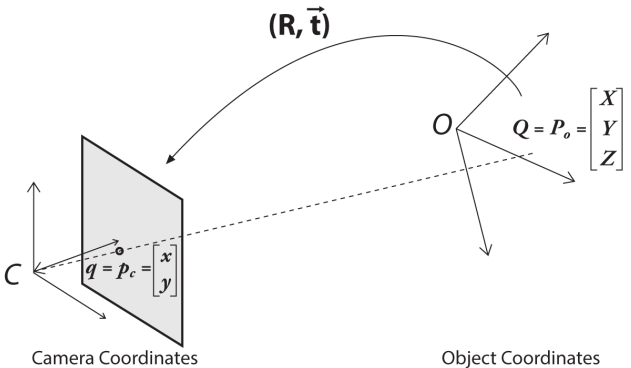
\includegraphics[width=3cm]{Figs/rot_trans.png}}}
\end{tabular}
\end{center}
\caption{O objetivo é matematicamente alinhar as duas câmeras em um plano de visão, de forma que as imagens fiquem exatamente alinhadas e a busca por pixels fique mais restrita. }
\label{fig:req2}
\end{figure}

Para um ponto tridimensional $\overrightarrow{P}$ nas coordenadas do objeto, nós podemos separá-lo usando a calibração de uma única câmera para as duas câmeras. Assim, para por $\overrightarrow{P}$ nas coordenadas da câmera para cada câmera fazemos: $\overrightarrow{P_l} = {R_l} \cdot (\overrightarrow{P}) + \overrightarrow{T_l})$ e $\overrightarrow{P_r} = {R_r} \cdot (\overrightarrow{P}) + \overrightarrow{T_r})$.
As duas vistas deste ponto $\overrightarrow{P}$ (obtidas das duas câmeras) são relacionadas por $\overrightarrow{P_l} = {R^T} \cdot (\overrightarrow{P_r} - \overrightarrow{T} )$, onde $R$ e $\overrightarrow{T}$ são, respectivamente, a matriz de rotação e o vetor de translação entre as câmeras. Usando essas três equações é possível obter a rotação $R$ e a translação $\overrightarrow{T}$ que foi usada para a retificação das imagens do Morpheus: $$R = R_r \cdot {R_l}^T \, \mbox{e } \overrightarrow{T} = \overrightarrow{T_r} - R \cdot \overrightarrow{T_l}.$$
Aplicando o método para alinhar os planos da imagens descrito acima, que é conhecido como o algoritmo de Bouget apresentado em ~\cite{kaehler2016learning}, é obtida a configuração estéreo necessária. Os novos centros da imagens e as novas bordas são então escolhidas para as imagens rotacionadas, de forma a maximizar a área de visualização sobreposta. No contexto da biblioteca OpenCV, o algoritmo de Bouget é implementado pela função \textit{cv::stereoRectify()}~\cite{opencvmanual}. Para esta função é fornecido as matrizes das câmeras, o tamanho da imagem, $R$ e $\overrightarrow{T}$ calculados anteriormente. Os parâmetros de retorno são $R_l$, $R_r$ (as rotações para a retificação dos planos esquerdo e direito da imagem), $P_l$ e $P_r$ (matrizes 3x4 de projeção) e, por fim, a matriz de reprojeção $Q$.

O processo de retificação é então feito pela função \textit{cv::initUndistortRectifyMap()}, usando as saídas $R_l$, $R_r$, $P_l$ e $P_r$. Esta função é chamada duas vezes, uma para a imagem da esquerda e uma para a da direita. O processo de retificação é ilustrado na \textbf{Figura} \ref{fig:req2.2}. Como mostrado na equação da figura, o processo de retificação funciona de (c) para (a) em um processo conhecido como mapeamento reverso. Para cada pixel inteiro na imagem retificada (c), é encontrado as suas coordenadas na imagem sem distorção (b) e eles são usados para procurar as verdadeiras coordenadas (ponto flutuante) na imagem de origem (a). O valor da coordenada do pixel em ponto flutuante é então interpolado com os pixels vizinhos inteiros na imagem original, e este valor é usado para preencher a posição dos pixels inteiros retificados na imagem de destino (c).

\begin{figure}[h]
\begin{center}
\begin{tabular}{c}
\bmvaHangBox{\fbox{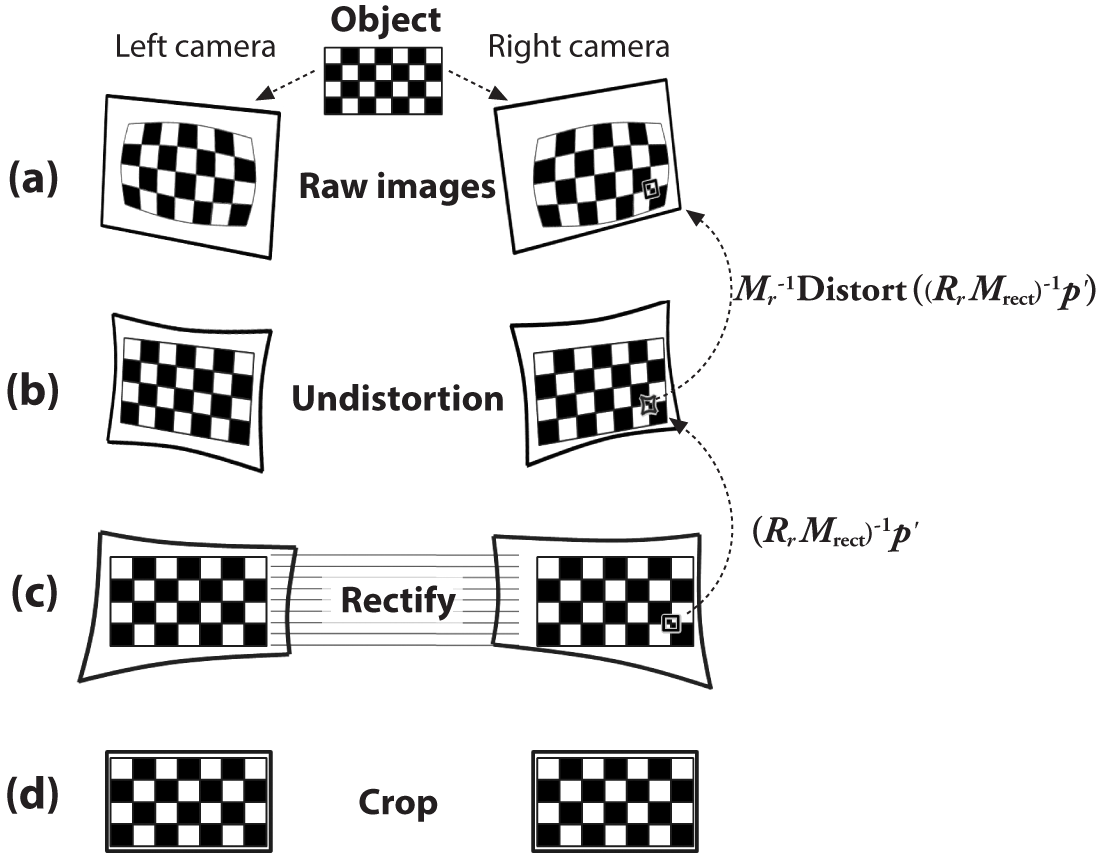
\includegraphics[width=2.5cm]{Figs/stereo_rectification.png}}}
\end{tabular}
\end{center}
\caption{Retificação estéreo para as imagens das câmeras da esquerda e da direita. }
\label{fig:req2.2}
\end{figure}

Depois da retificação é usada a função \textit{remap} para finalizar o processo de retificação e permitir a busca por elementos ao longo da mesma linha (mesma coordenada y) nas duas imagens. Os mapas de disparidade foram obtidos assim como no \ref{req1}, usando o SGBM.
\subsection{Requisito 3}
\label{Met:Req4}
Pontos em duas dimensões podem ser reprojetados em três dimensões dados as coordenadas das câmeras e a matriz intrínseca da câmera. A matriz de reprojeção $Q$ é: $$ \begin{bmatrix}
1 & 0 & 0 & -c_x \\
0 & 1 & 0 & -c_y \\
0 & 0 & 0 & f \\
0 & 0 & \frac{-1}{T_x} & \dfrac{c_x - {c_x}^{'}}{T_x} 
\end{bmatrix}  $$
Os parâmetros são da imagem da esquerda, exceto por ${c_x}^{'}$, que é o ponto principal na coordenada x da imagem da direita. Se os raios principais se cruzam no infinito, então ${c_x}^{'} = c_x$. Dado um ponto bidimensional homogêneo e sua disparidade associada $d$, nós podemos projetar o ponto em 3D usando a matriz $Q$, conforme a função da OpenCV utilizada: \textit{reprojectImageTo3D()}.

Após os pontos terem sido projetados nas coordenadas do mundo real, foi calculado a norma entre eles para obter as medidas pedidas.
%-------------------------------------------------------------------------
\section{Resultados}
\label{sec:Results}
Nesta seção são apresentados em forma de figuras e tabelas os resultados da aplicação para cada um dos requisitos. 
%-------------------------------------------------------------------------
\subsection{Requisito 1}
\label{aloebaby}
As imagens da \textbf{Figura} \ref{res:req1} e \ref{res:req1.2} mostram a comparação do algoritmo BM e SGBM para calcular os mapas de disparidade e profundidade na imagem \textit{baby} e \textit{aloe}.
\begin{figure}[h]
\begin{center}
\begin{tabular}{cccc}
\bmvaHangBox{\fbox{\parbox{2.5cm}{
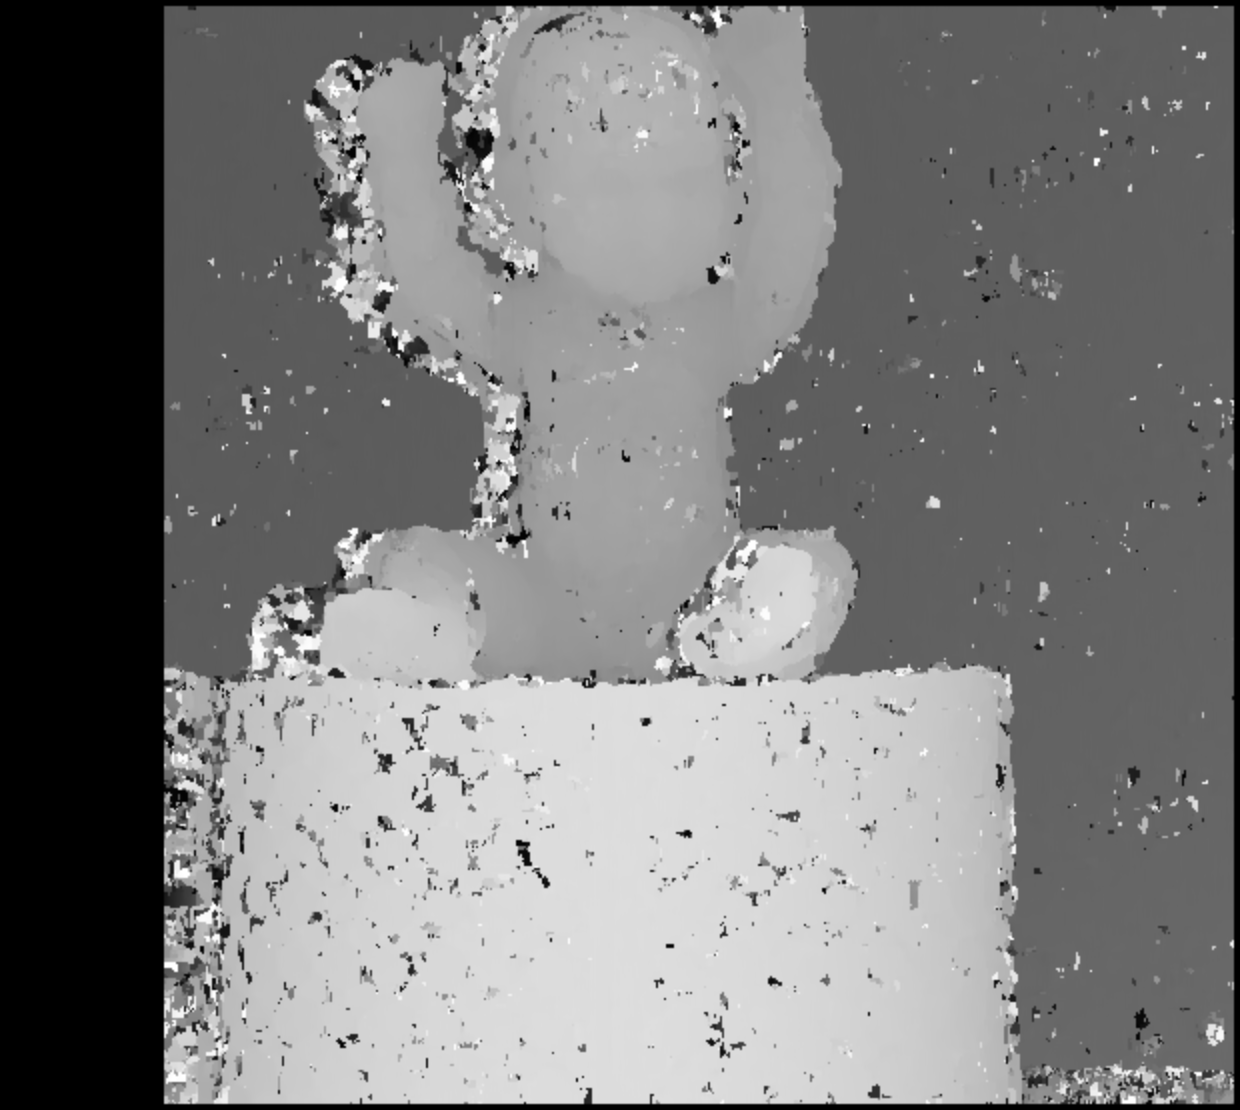
\includegraphics[width=2.5cm]{Figs/baby_bm_disp.png}}}} &
\bmvaHangBox{\fbox{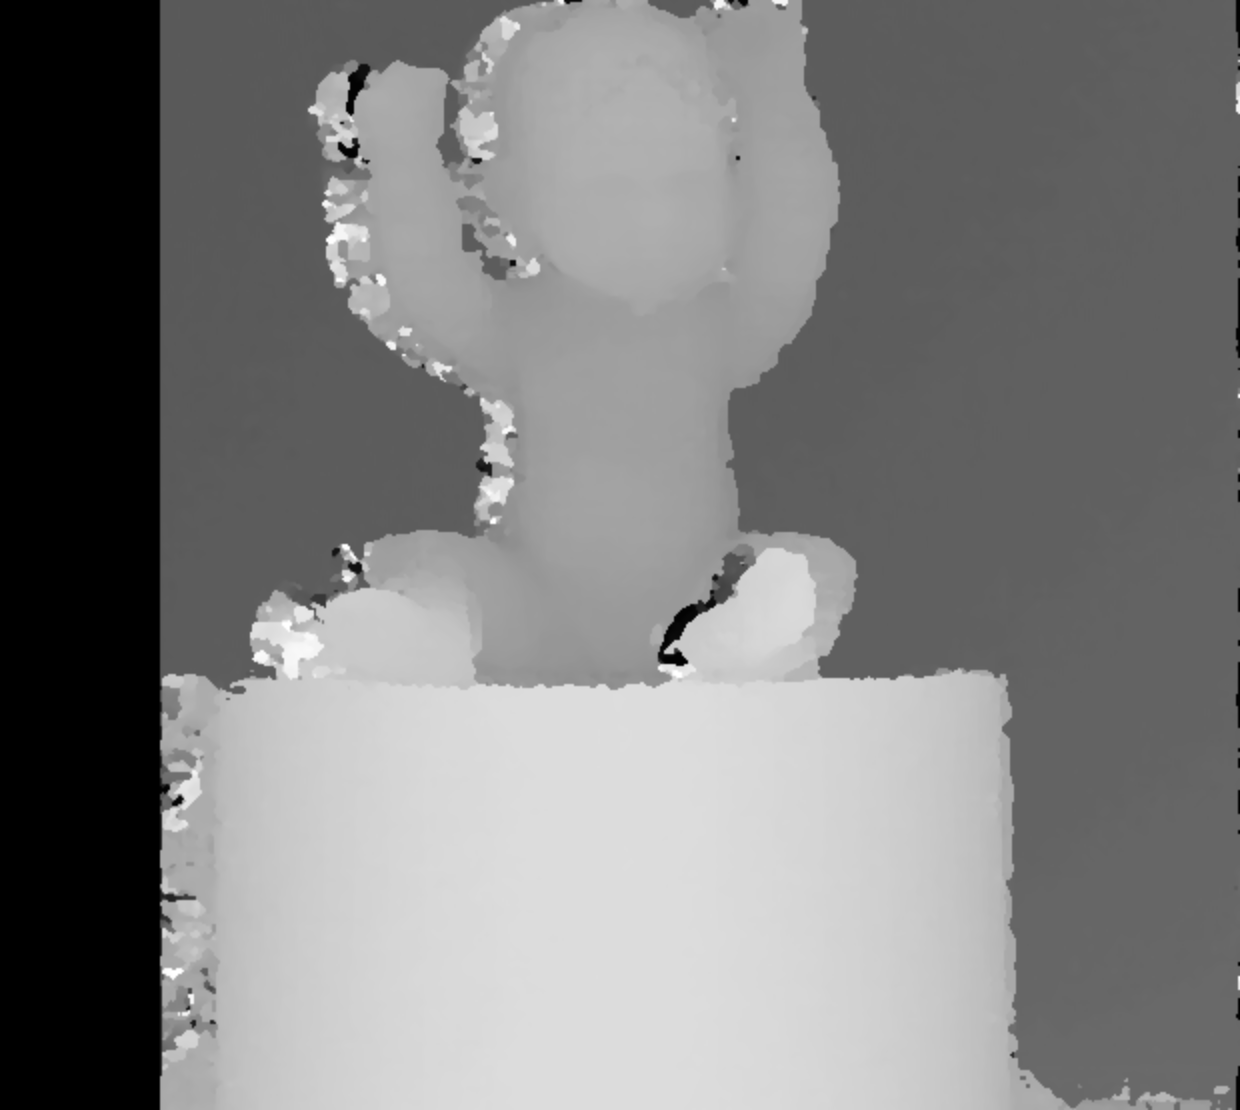
\includegraphics[width=2.5cm]{Figs/baby_sgbm_disp.png}}} &
\bmvaHangBox{\fbox{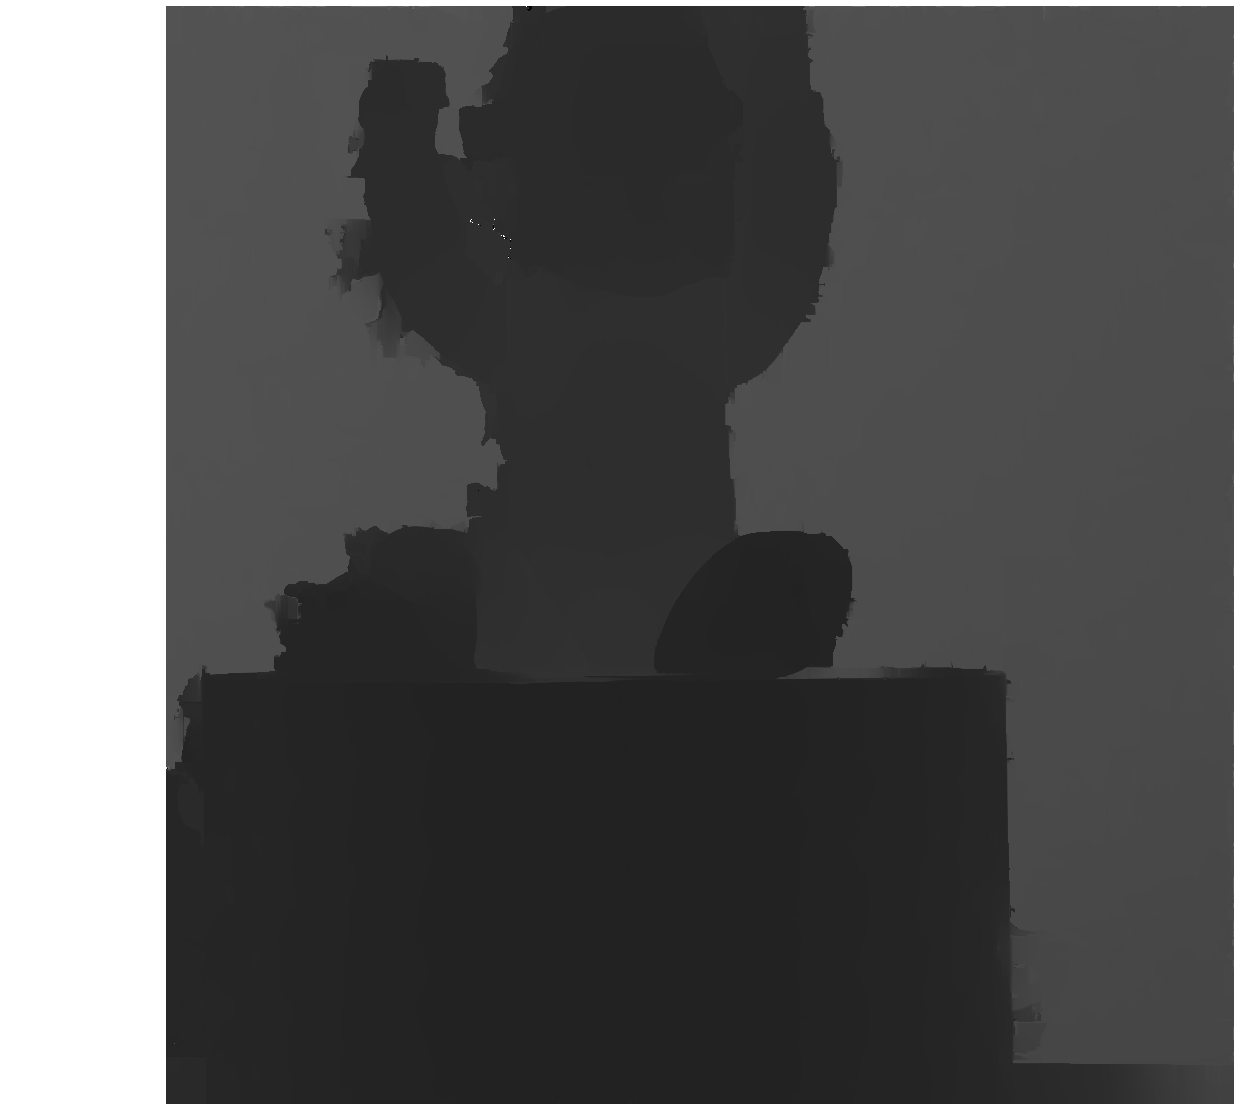
\includegraphics[width=2.5cm]{Figs/baby_bm_depth.png}}} &
\bmvaHangBox{\fbox{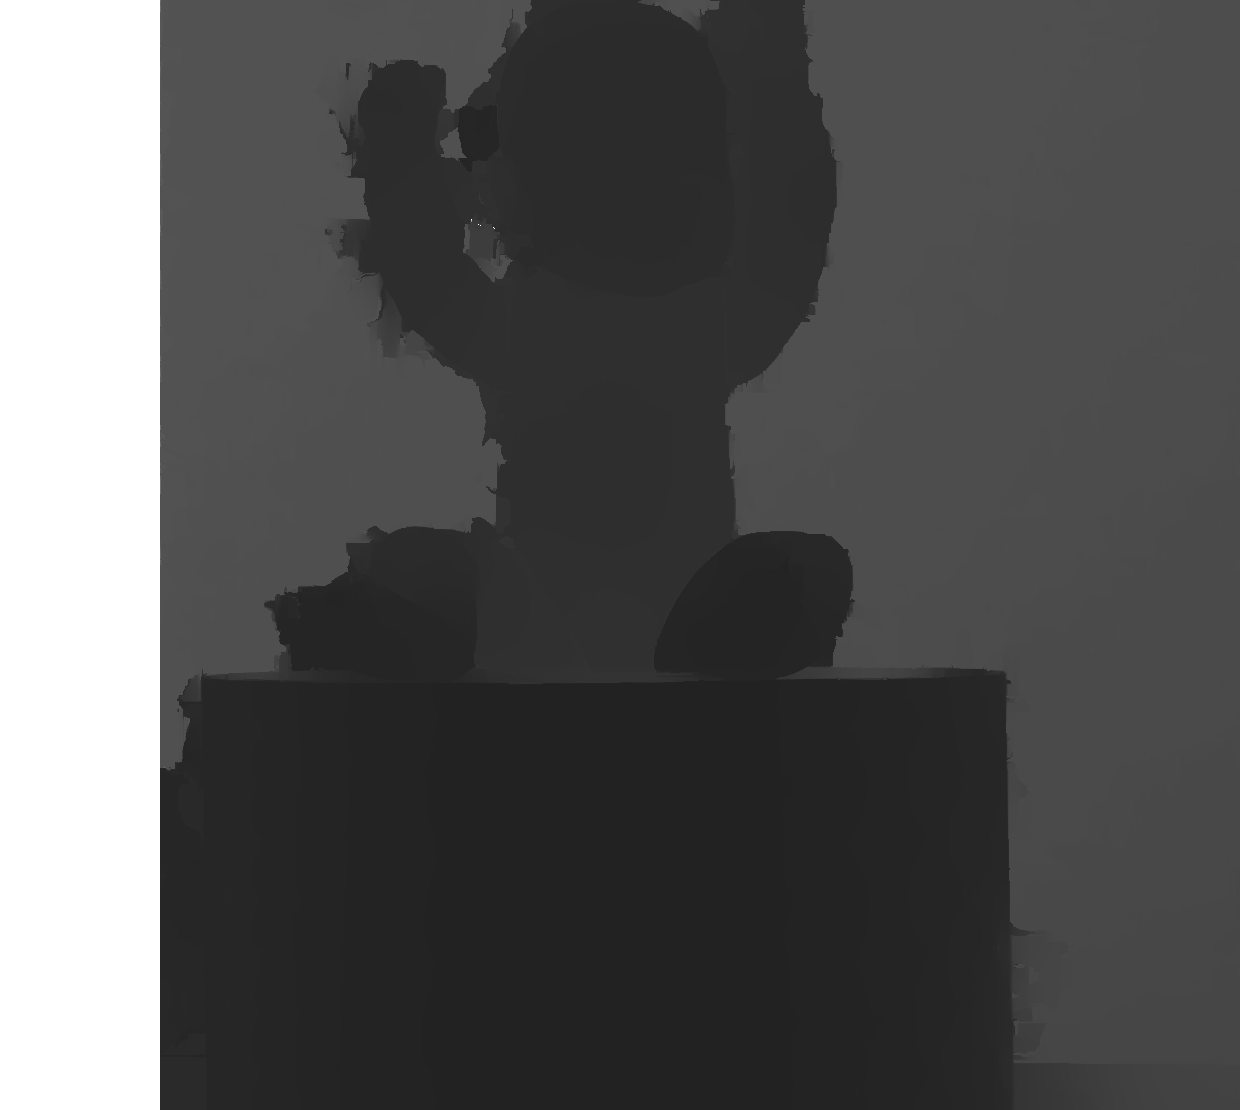
\includegraphics[width=2.5cm]{Figs/baby_sgbm_depth.png}}} \\
(a)&(b)&(c)&(d)
\end{tabular}
\end{center}
\caption{(a), (b), (c) e (d) são as imagens de disparidade usando bm e sgbm e as imagens de profundidade usando bm e sgbm, respectivamente.}
\label{res:req1}
\end{figure}

\begin{figure}[h]
\begin{center}
\begin{tabular}{cccc}
\bmvaHangBox{\fbox{\parbox{2.5cm}{
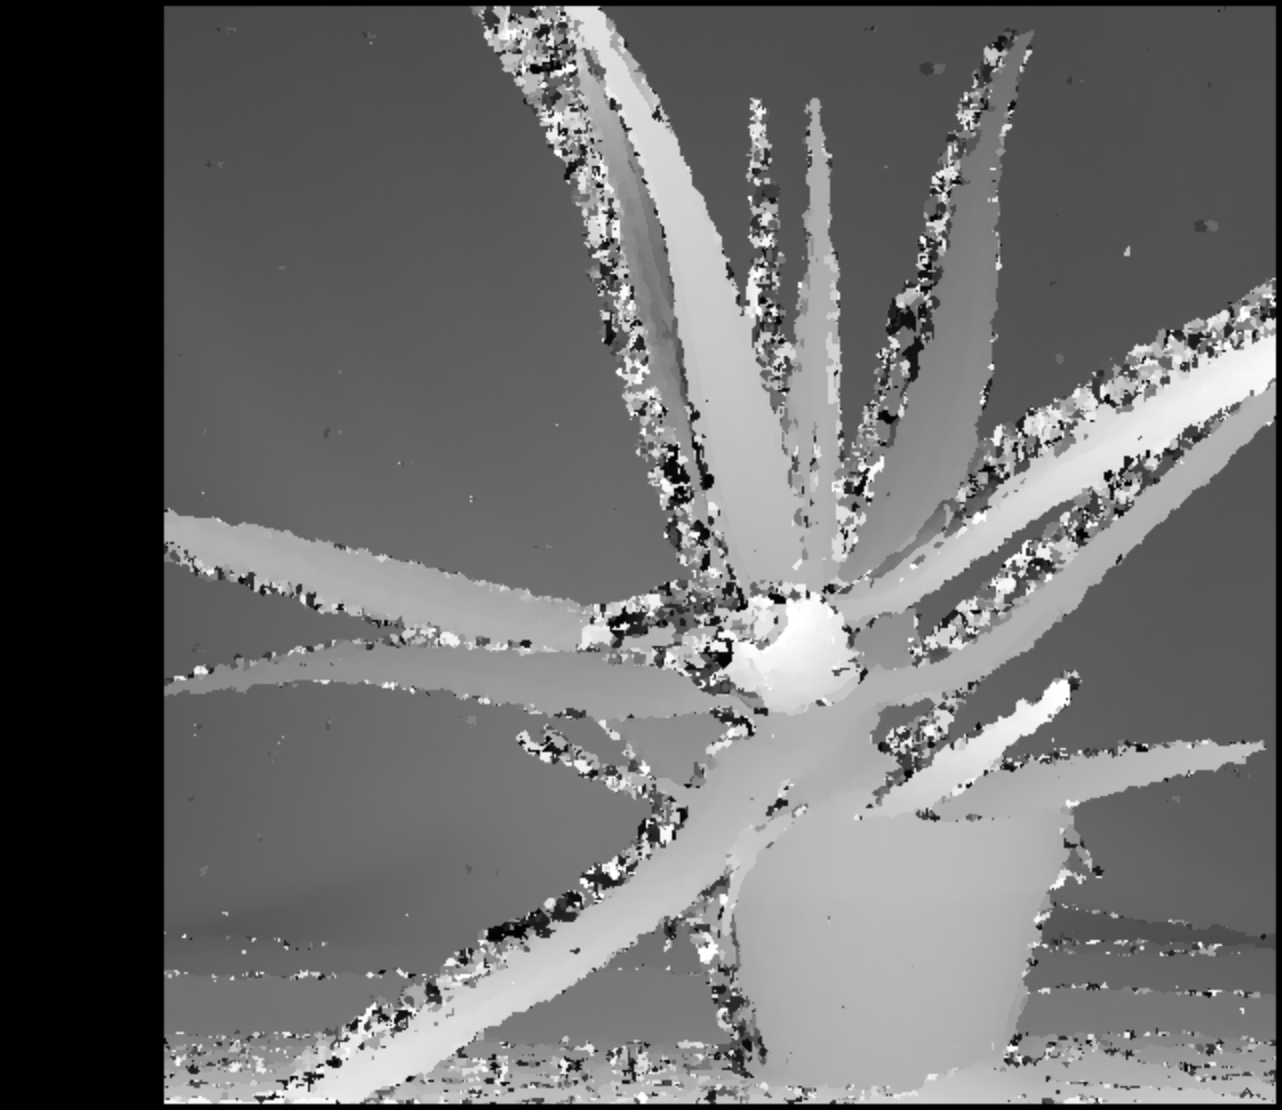
\includegraphics[width=2.5cm]{Figs/aloe_bm_disp.png}}}} &
\bmvaHangBox{\fbox{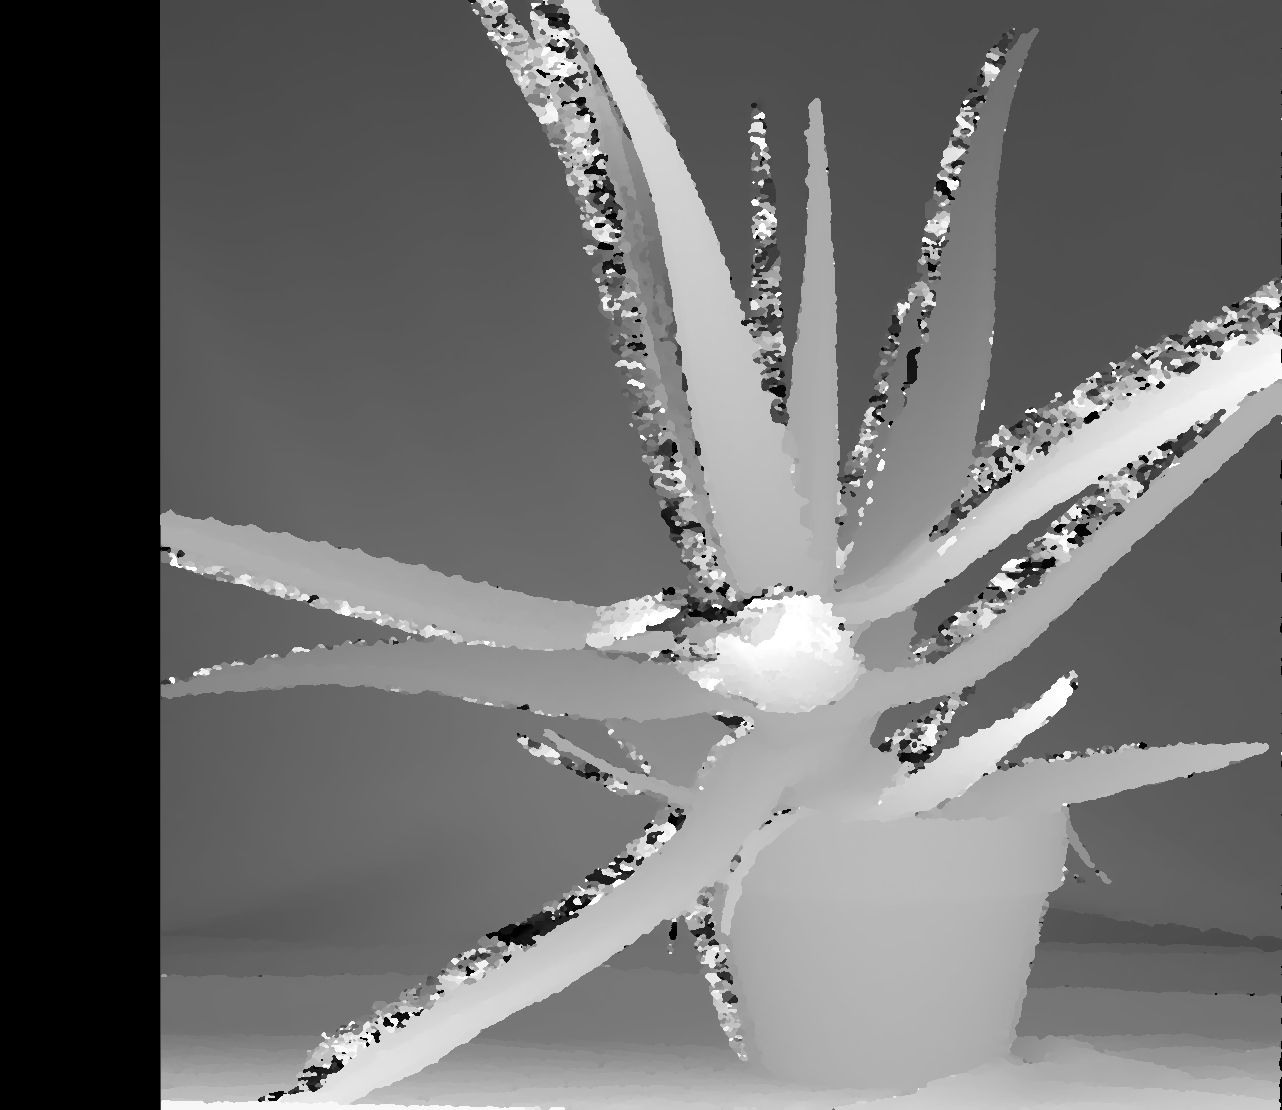
\includegraphics[width=2.5cm]{Figs/aloe_sgbm_disp.png}}} &
\bmvaHangBox{\fbox{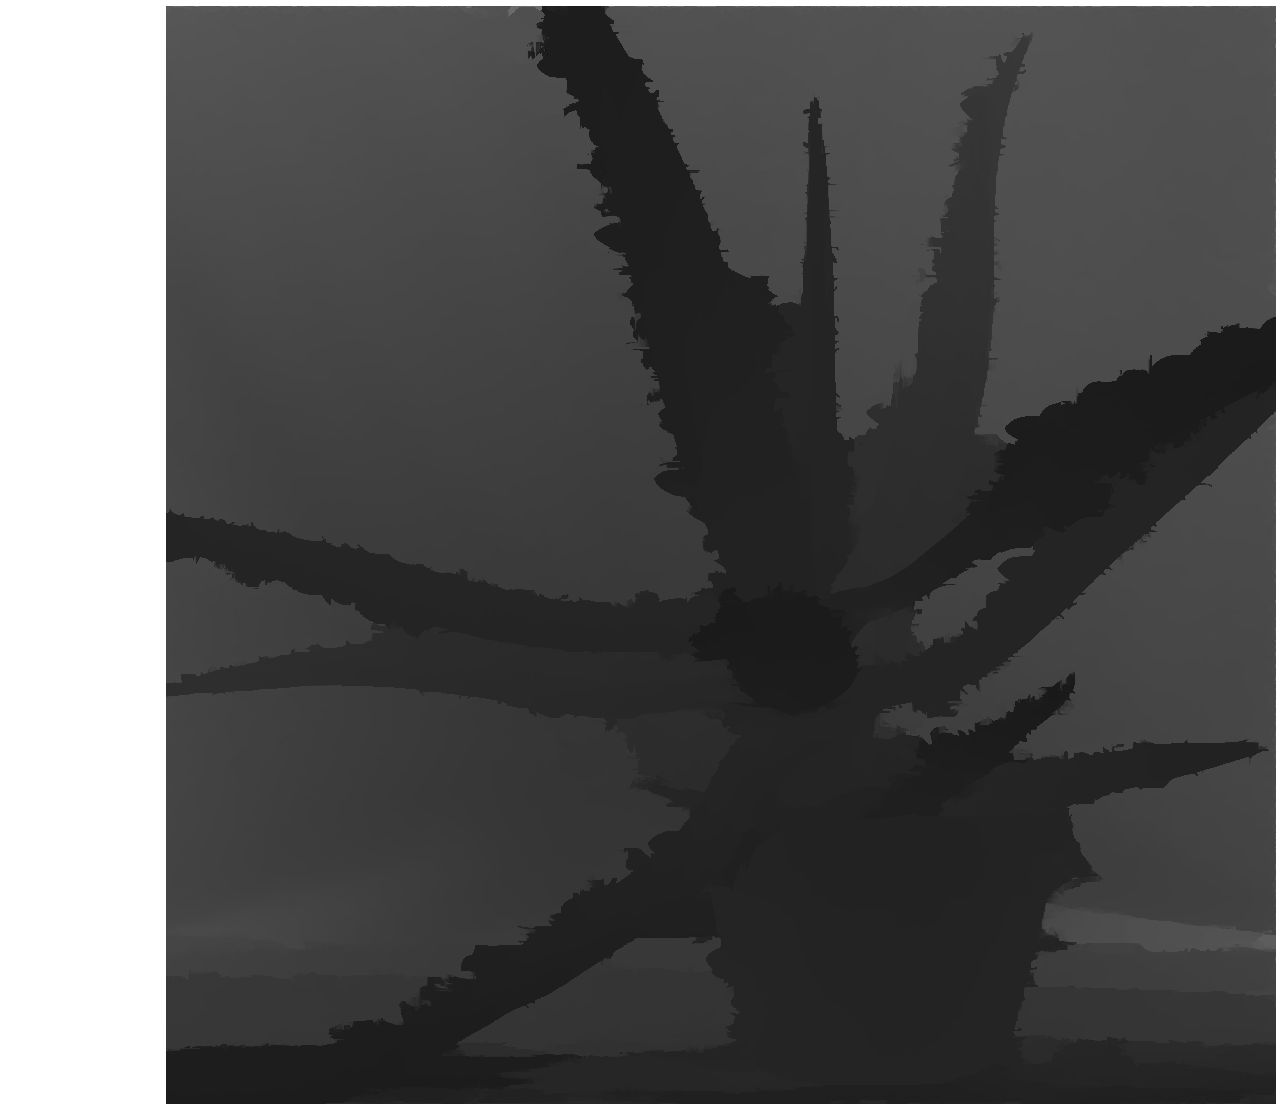
\includegraphics[width=2.5cm]{Figs/aloe_bm_depth.png}}} &
\bmvaHangBox{\fbox{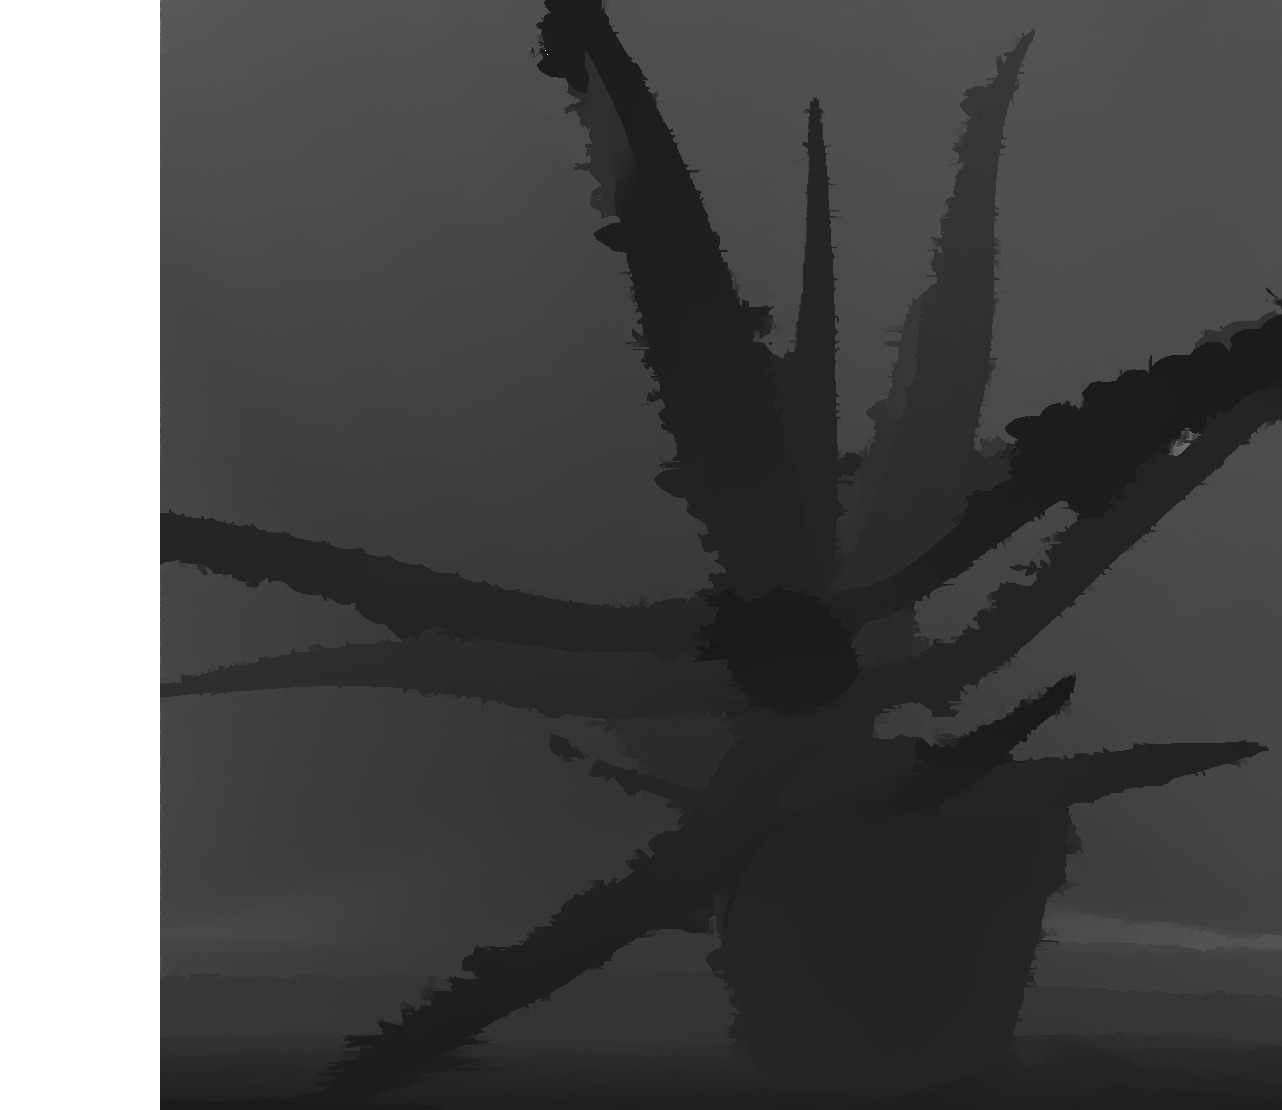
\includegraphics[width=2.5cm]{Figs/aloe_sgbm_depth.png}}} \\
(a)&(b)&(c)&(d)
\end{tabular}
\end{center}
\caption{(a), (b), (c) e (d) são as imagens de disparidade usando bm e sgbm e as imagens de profundidade usando bm e sgbm, respectivamente.}
\label{res:req1.2}
\end{figure}

Conforme mostra a \textbf{Tabela} \ref{table}, o SGBM teve um tempo de execução mais de 20 vezes superior ao BM para que a correspondência/casamento entre os pontos apresentada em \ref{req1} fosse realizada, o que já era esperado.
\begin{table}[h]
\centering
\label{table}
\caption{Tabela de comparação BM x SGBM.}
\begin{tabular}{|c|c|c|}
\hline
               & \textbf{Baby}                                                                              & \textbf{Aloe}                                                                              \\ \hline
\textbf{BM}    & \textbf{\begin{tabular}[c]{@{}l@{}}Correspondência:  0.22s\\ Filtragem: 0.1s\end{tabular}} & \textbf{\begin{tabular}[c]{@{}l@{}}Correspondência: 0.15s\\ Filtragem: 0.09s\end{tabular}} \\ \hline
\textbf{SGBM} & \textbf{\begin{tabular}[c]{@{}l@{}}Correspondência: 3.6s\\ Filtragem: 0.095s\end{tabular}} & \textbf{\begin{tabular}[c]{@{}l@{}}Correspondência: 3.8s\\ Filtragem: 0.096s\end{tabular}} \\ \hline
\end{tabular}
\end{table}

%-------------------------------------------------------------------------
\subsection{Requisito 2}
%-------------------------------------------------------------------------
Como pode-se notar pela \textbf{Figura} \ref{pair}, a retificação estéreo explicada em \ref{Methods:req2} foi feita com sucesso. Ou seja, as imagens estão alinhadas e os planos de projeção ficaram paralelos de modo que um pixel de um elemento da imagem esquerda está, na teoria, ``alinhado'' com o mesmo pixel no mesmo elemento da imagem direita. Assim, a busca por elementos correspondentes nas imagens se tornou bem mais restrita.

\begin{figure}[h]
\begin{center}
\begin{tabular}{cc}
\bmvaHangBox{\fbox{\parbox{4.5cm}{
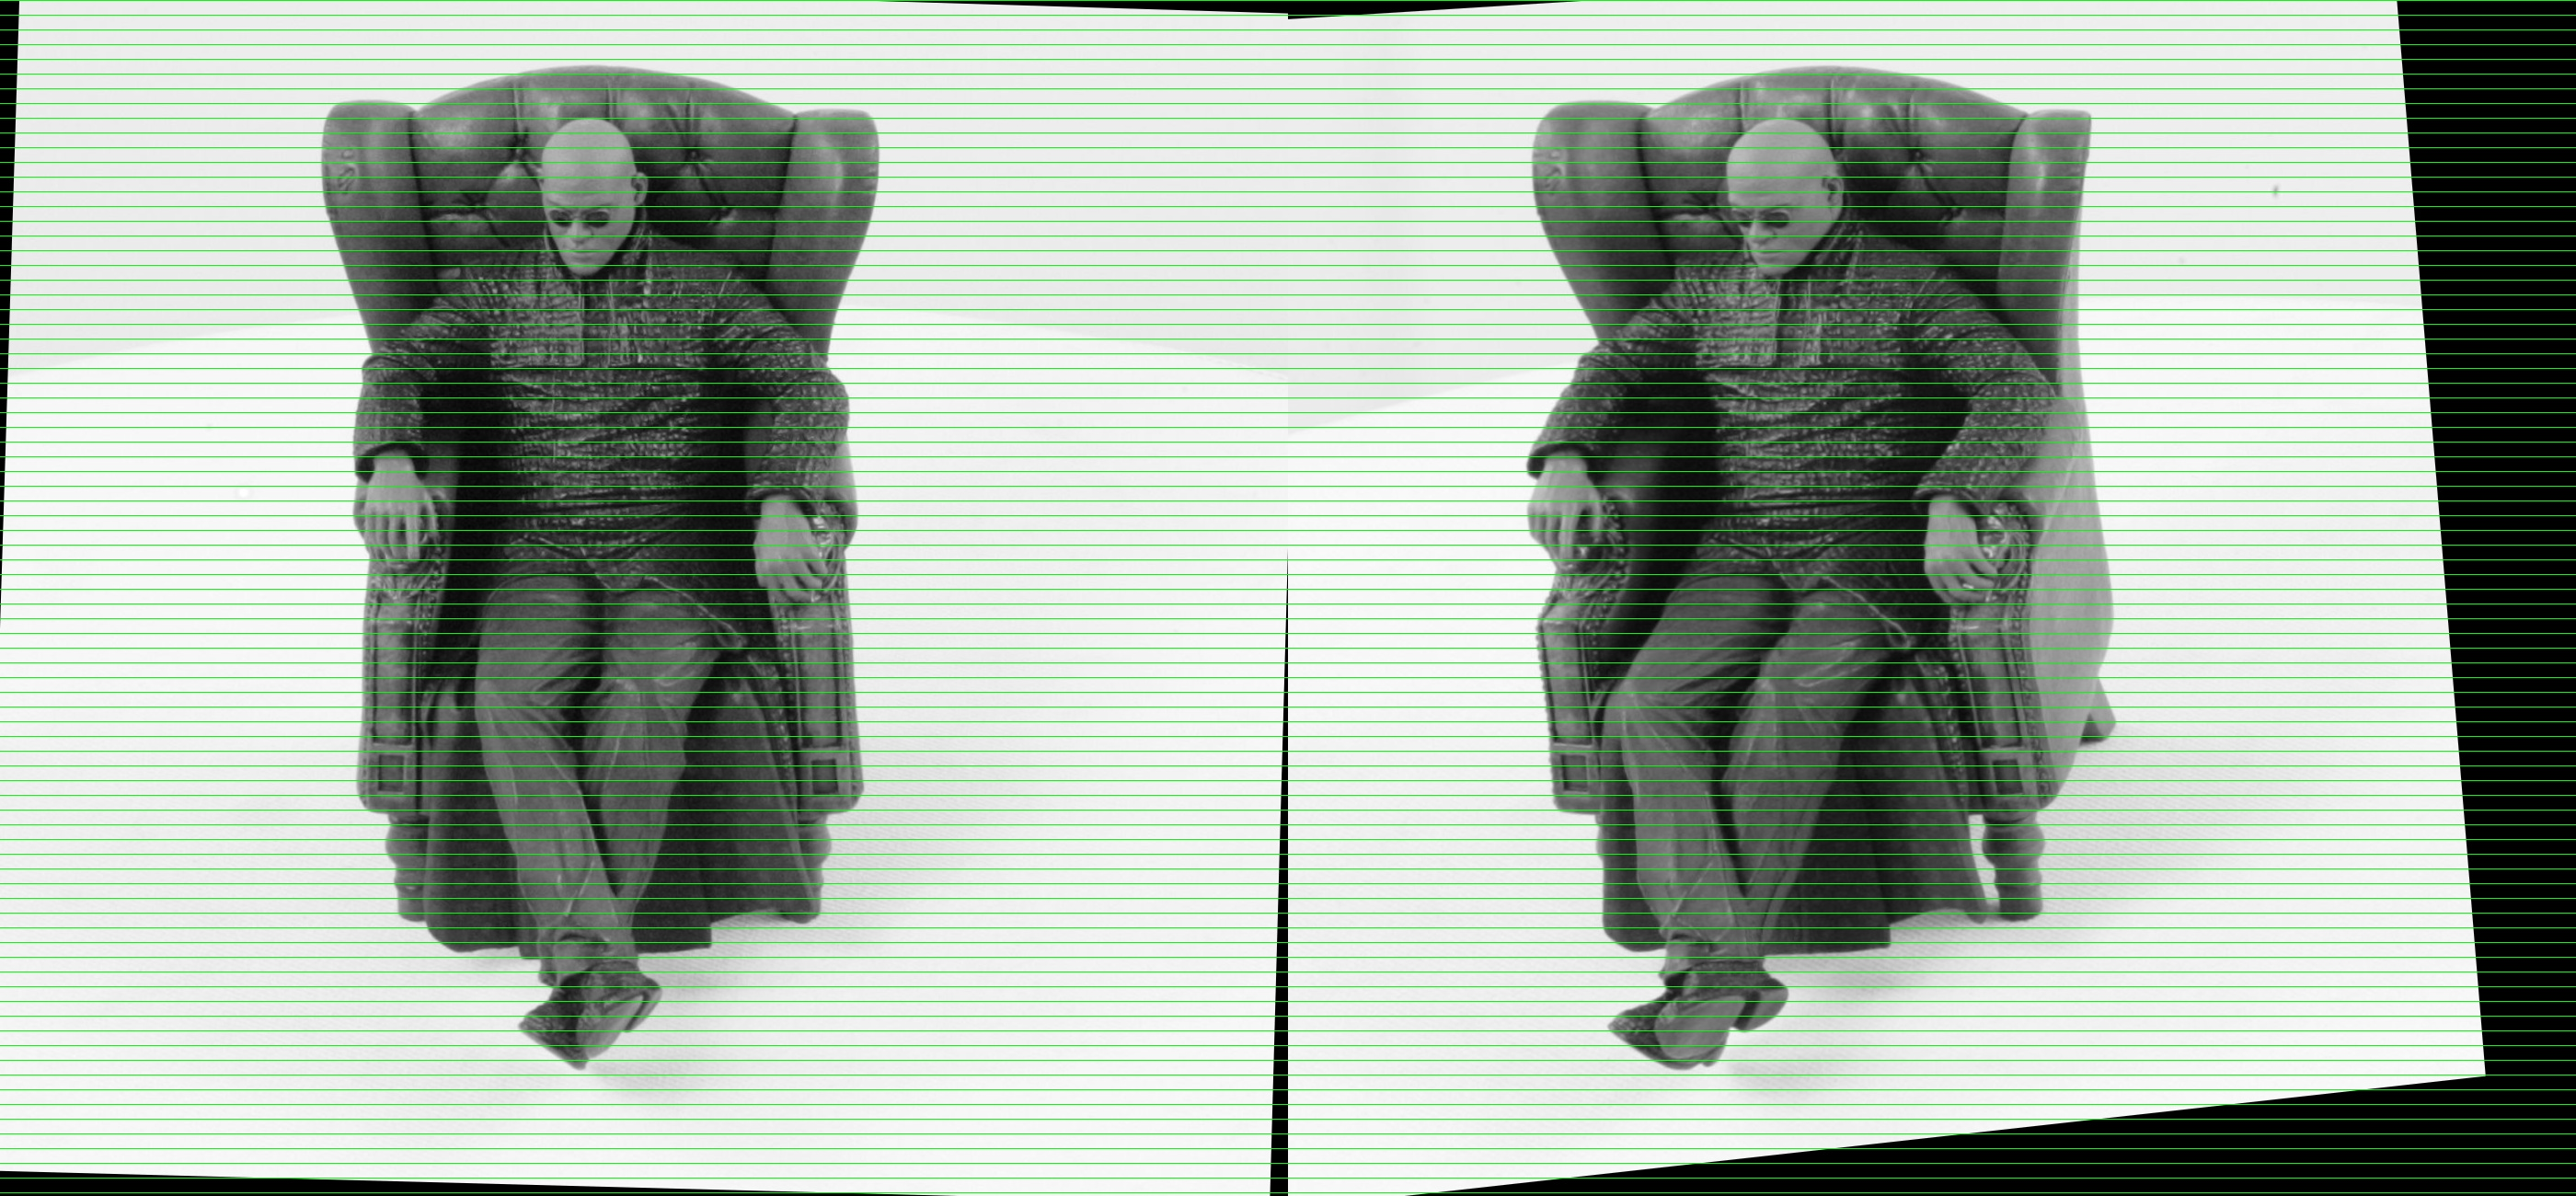
\includegraphics[width=4.5cm]{Figs/pair.jpg}}}} &
\bmvaHangBox{\fbox{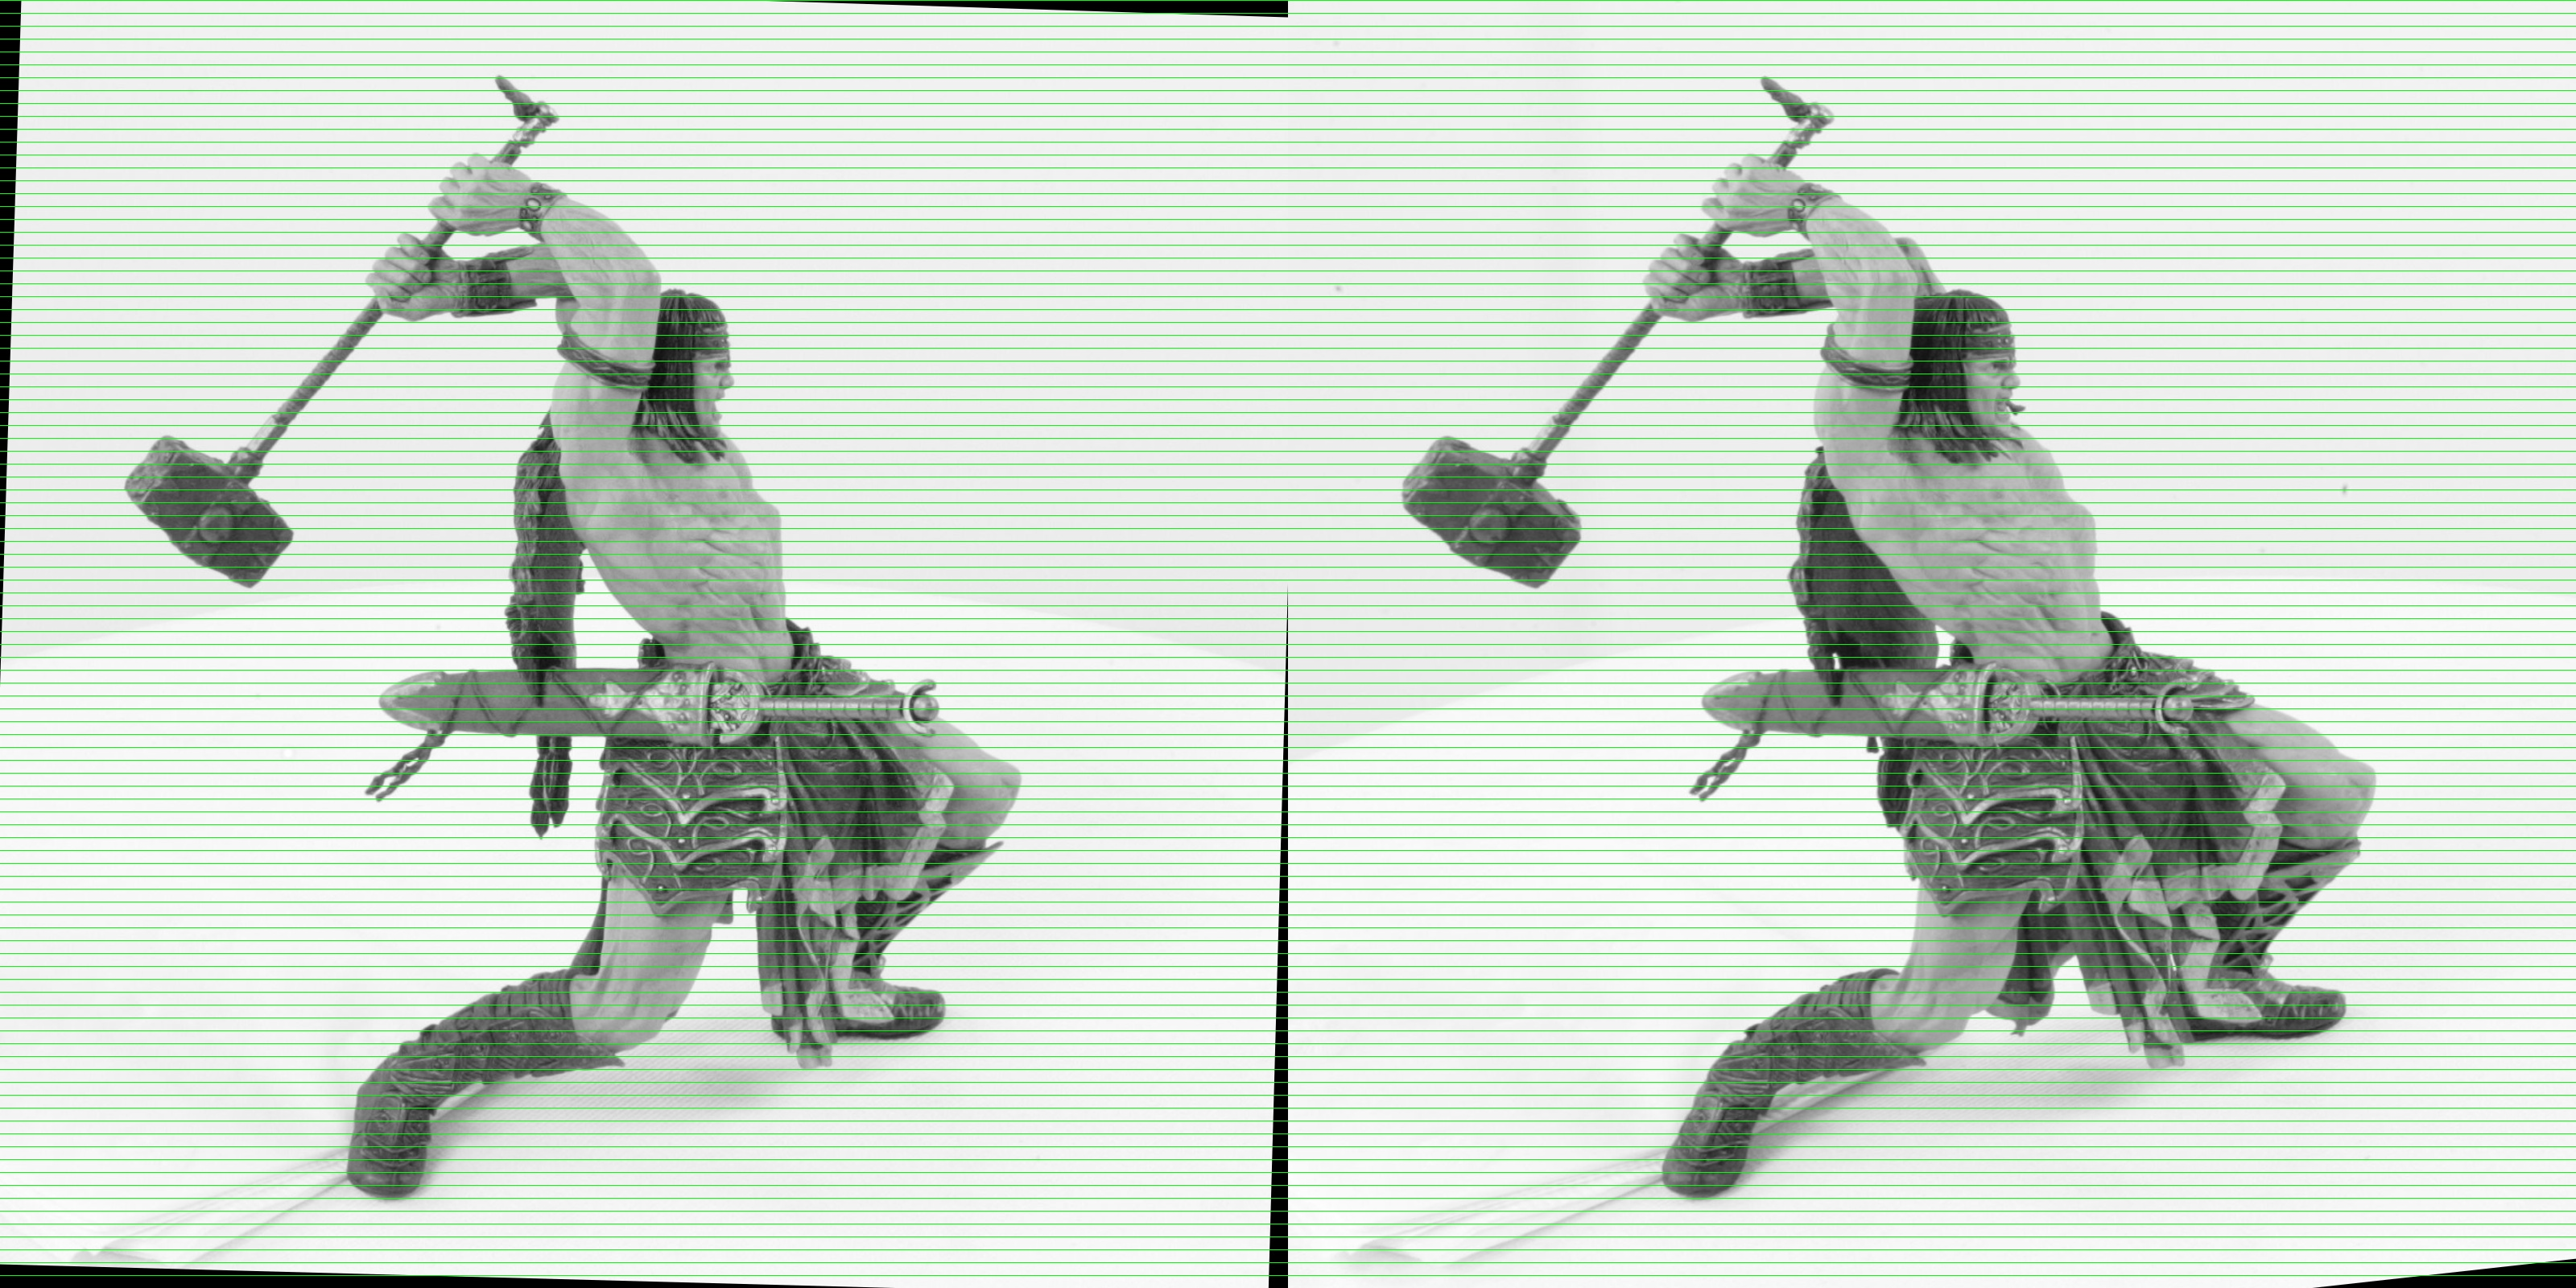
\includegraphics[width=4.5cm]{Figs/pair_warrior.jpg}}}
\end{tabular}
\end{center}
\caption{Imagens do morpheus e do warrior retificadas e alinhadas.}
\label{pair}
\end{figure}

A \textbf{Figura} \ref{morpheus} apresenta a disparidade e profundidade do Morpheus e do Warrior.
\begin{figure}[]
\begin{center}
\begin{tabular}{cccc}
\bmvaHangBox{\fbox{\parbox{2.5cm}{
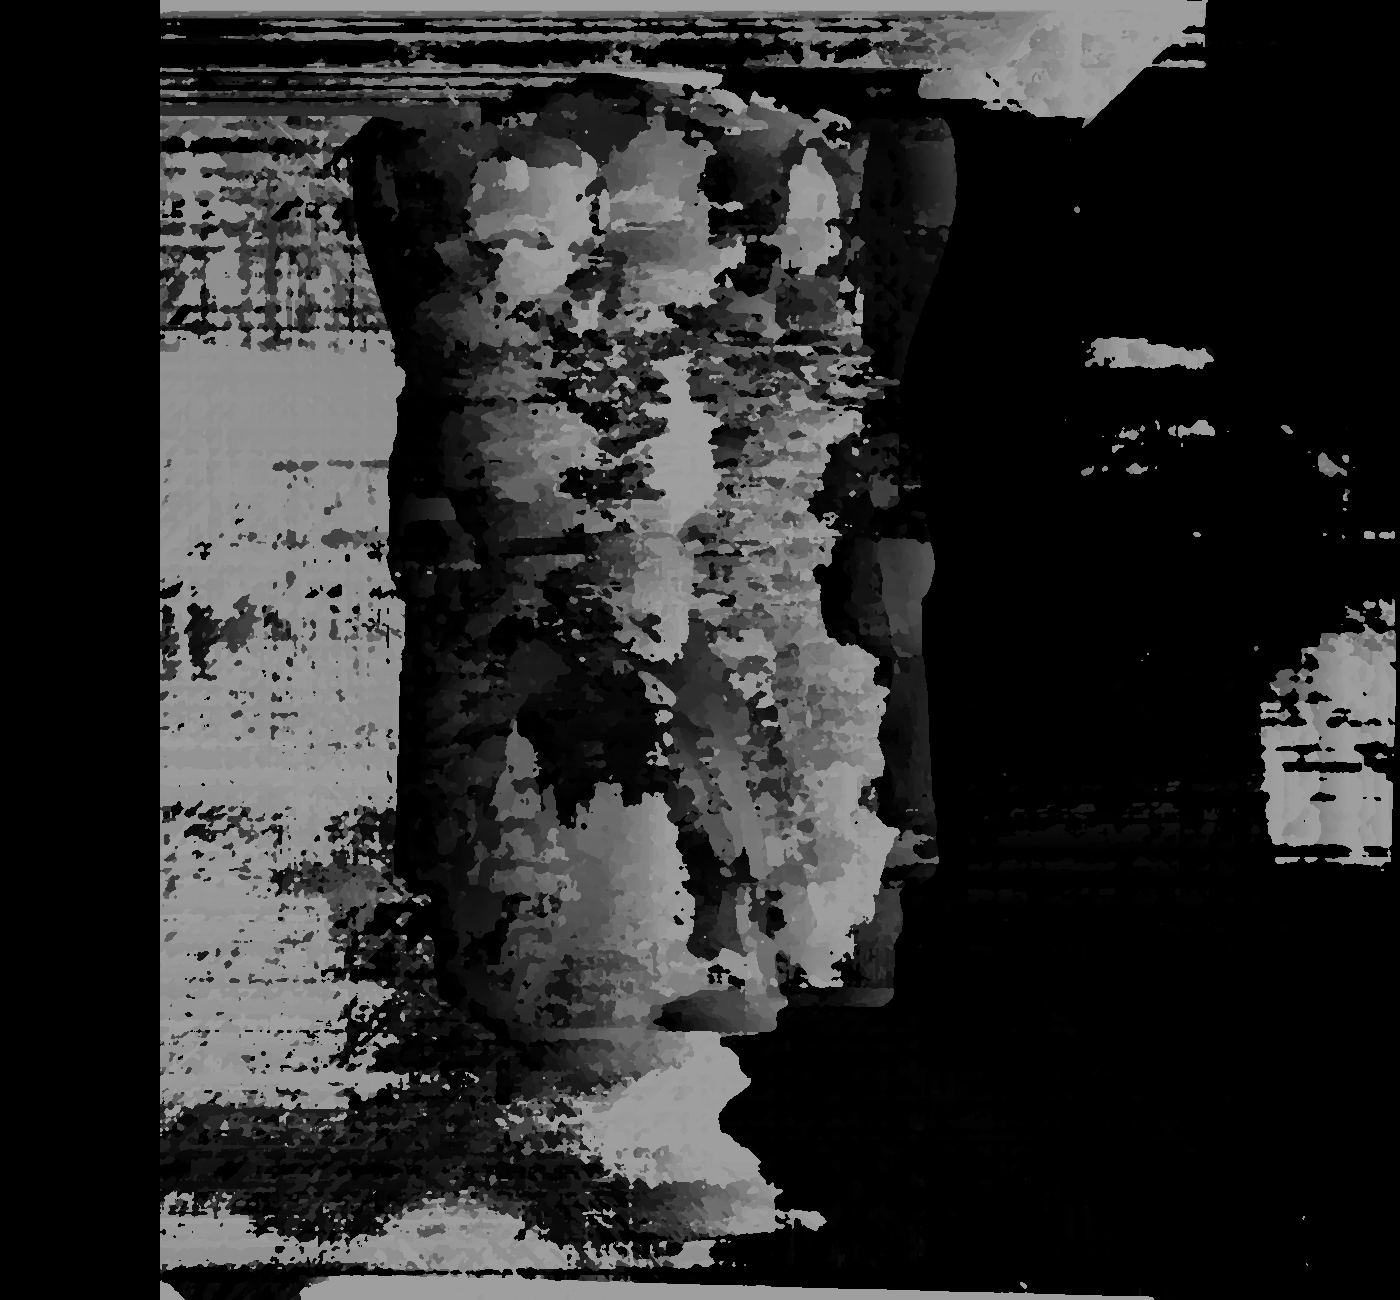
\includegraphics[width=2.5cm]{Figs/morpheus_disp.png}}}} &
\bmvaHangBox{\fbox{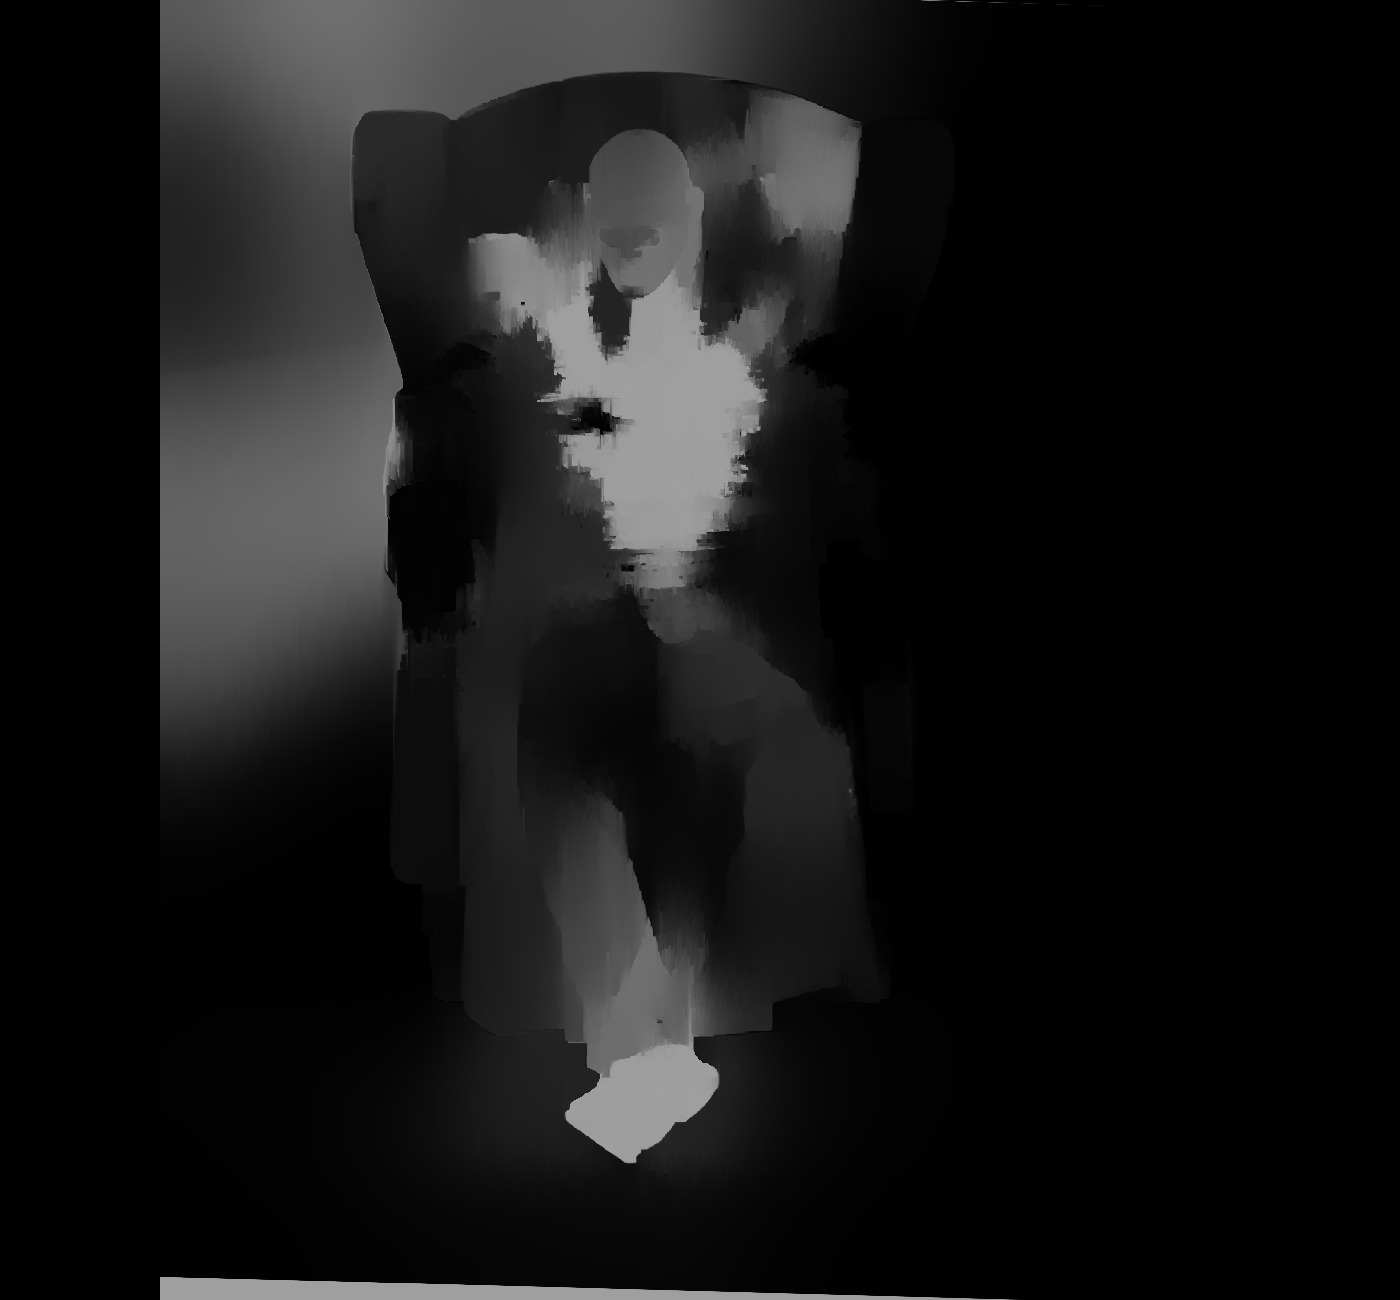
\includegraphics[width=2.5cm]{Figs/morpheus_depth.png}}} &
\bmvaHangBox{\fbox{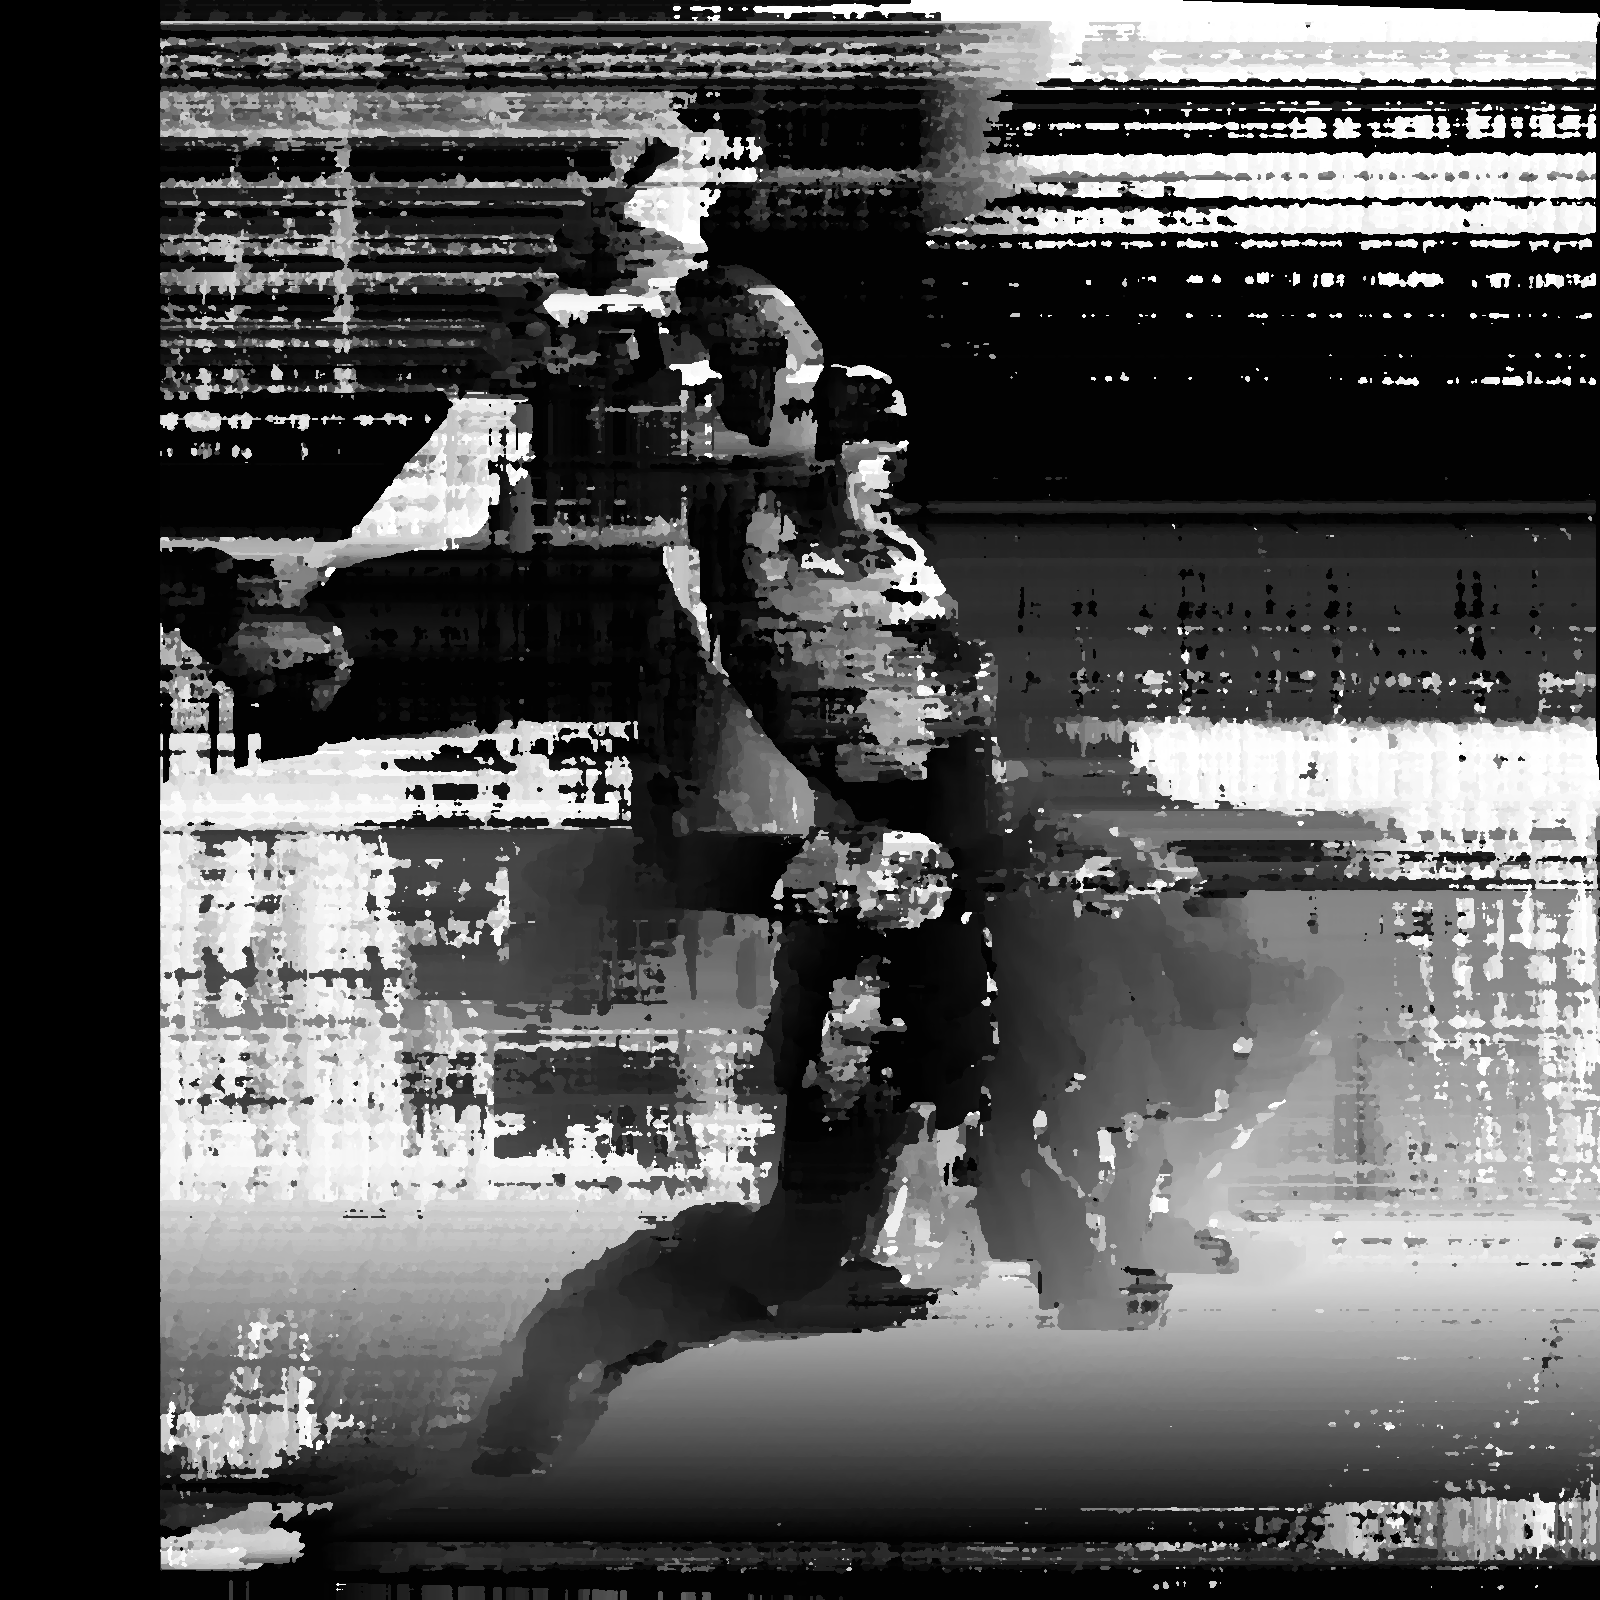
\includegraphics[width=2.5cm]{Figs/warrior_disp.png}}} &
\bmvaHangBox{\fbox{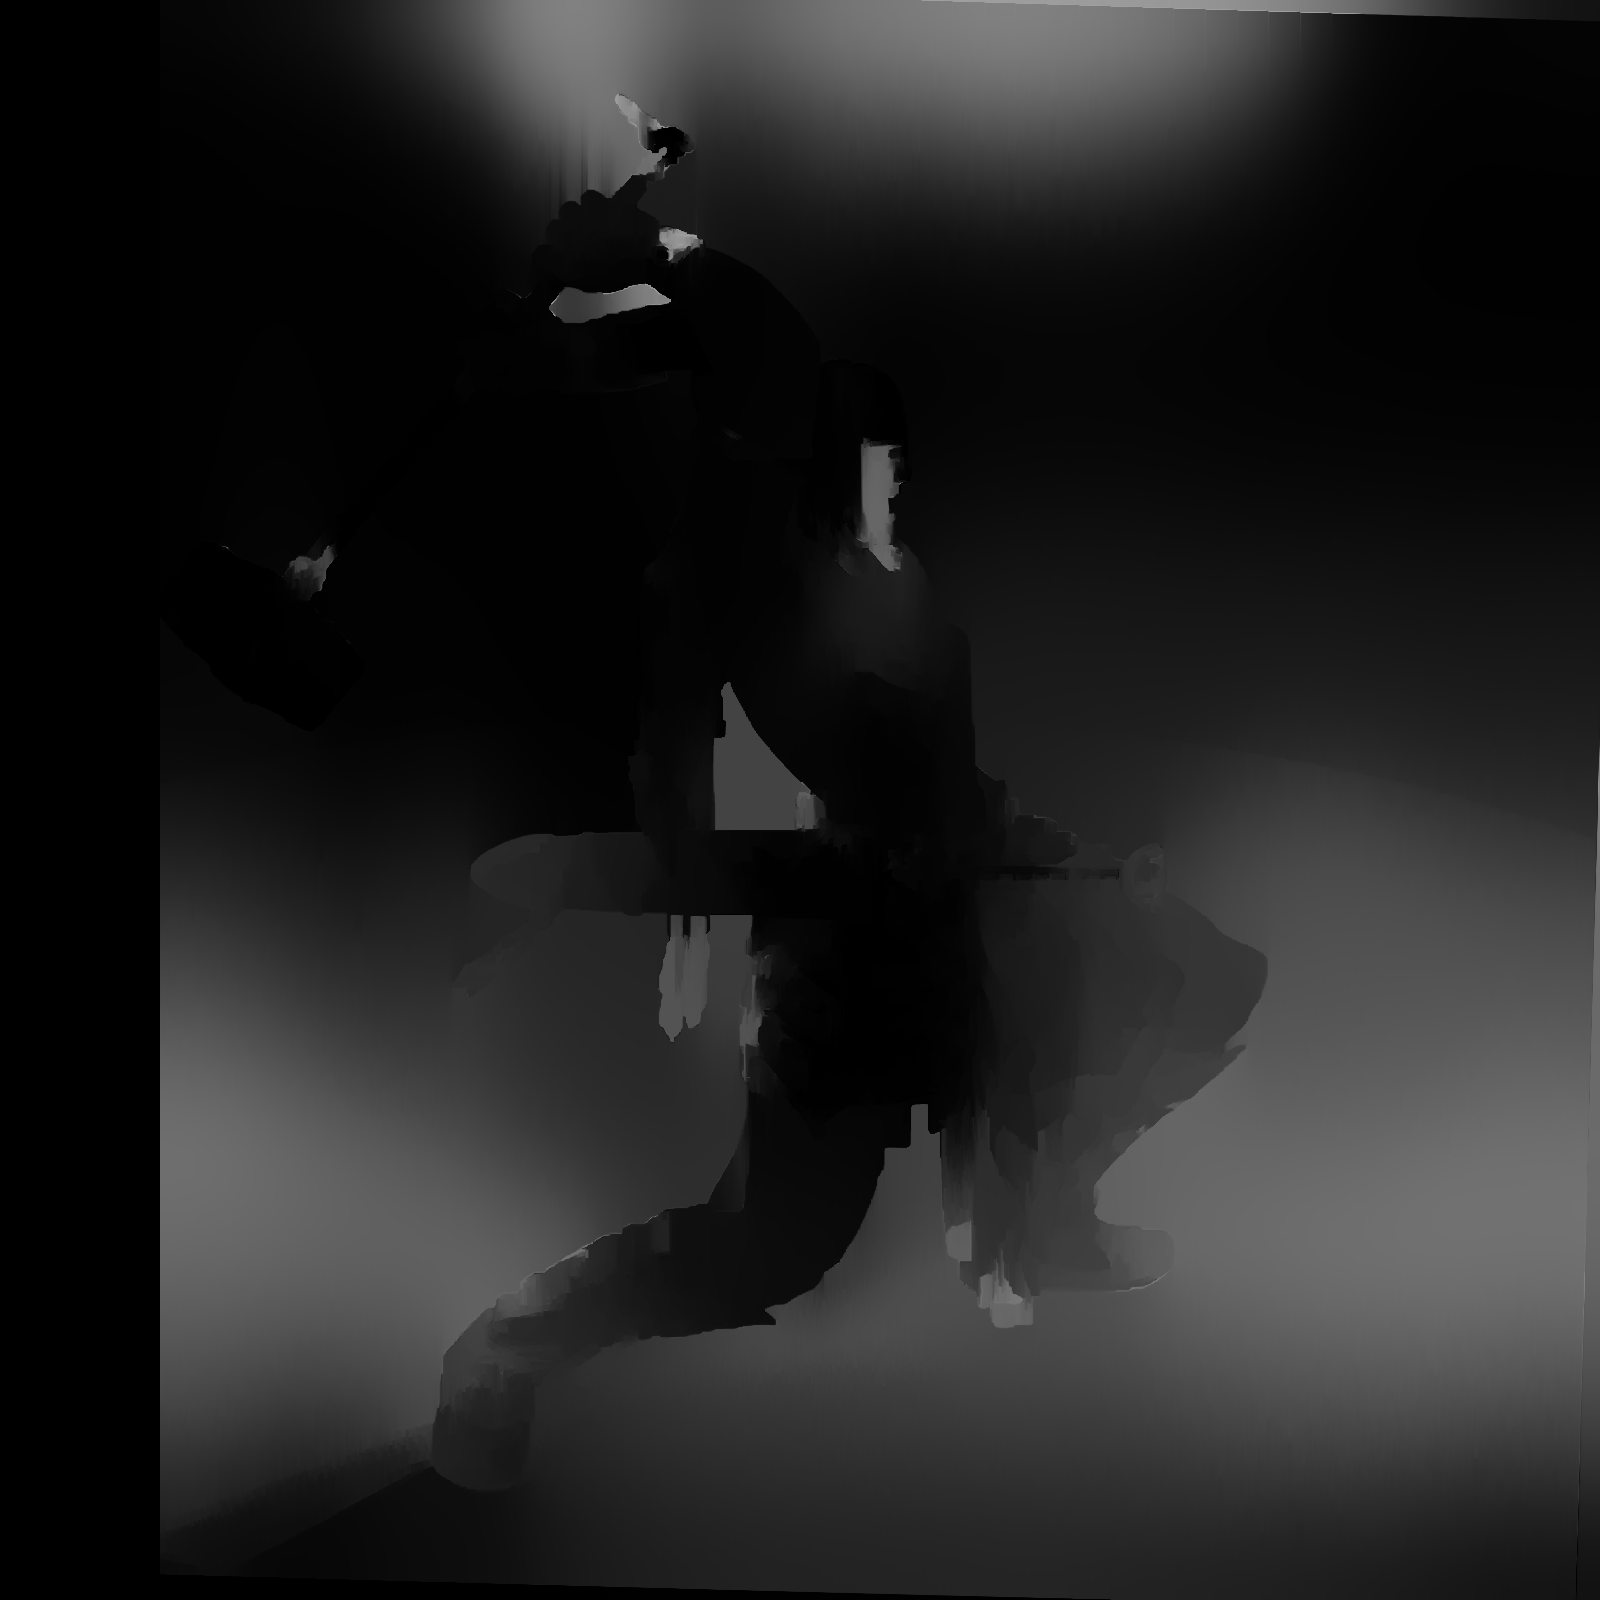
\includegraphics[width=2.5cm]{Figs/warrior_depth.png}}} \\
(a) & (b) & (c) & (d)
\end{tabular}
\end{center}
\caption{(a) e (b) são as imagens de disparidade e profundidade obtidas para o Morpheus, respectivamente. Assim como (c) e (d) são as do Warrior.}
\label{morpheus}
\end{figure}

\subsection{Requisito 3}
%-------------------------------------------------------------------------
As dimensões para a caixa (largura, altura e profundidade) obtidas foram, respectivamente: 15.1407 x 21.6495 x 9.45939 cm. Elas foram obtidas primeiro medindo a largura a partir do canto superior esquerdo do sofá, depois medindo a altura partindo do mesmo ponto, e por fim a profundidade foi obtida a partir da diagonal, clicando primeiro no canto inferior direito e depois no canto superior direito.
%-------------------------------------------------------------------------
\section{Discussões, Conclusões e Análise de Parâmetros}
\label{sec:Conclusion}
%-------------------------------------------------------------------------
Pode-se notar pela \textbf{Figura} \ref{res:req1} e \ref{res:req1.2} que o SGBM de fato cumpriu com o que prometeu e forneceu maior robustez e acurácia nos resultados, comparado ao mais velho BM, apesar do mapa de profundidade não ter tantas diferenças aparentes. No mapa de profundidade, ao contrário do mapa de disparidade, pixels mais escuros significam uma maior proximidade do elemento da imagem para a câmera.

Conforme dito anteriormente, no BM a correspondência é computada deslizando a janela SAD (soma das diferenças absolutas) nas imagens e no SGBM é usada um bloco com uma métrica de diferença absoluta dos sinais. Para cada característica na imagem da esquerda, nós procuramos a linha correspondente na imagem da direita por um melhor casamento. Depois da retificação, cada linha é uma linha epipolar de modo que a posição correspondente do ponto procurado na imagem da direita deve estar na mesma linha (mesma coordenada y) da imagem da esquerda. Esta posição pode ser encontrada se possui textura suficiente para ser detectável e se não está oculto na visão da câmera da direita. As posições não encontradas observadas nos mapas de disparidade apresentados em \ref{sec:Results} são justamente aquelas que não satisfazem estas duas condições. Isso vale, principalmente, para as imagens do morpheus, onde há mais regiões ocultas e uniformes. Nestas regiões uniformes (cenas com pouca textura), poucos pontos registraram profundidade. Enquanto em regiões com maior textura, muitos pixels registraram profundidade.

Além disso, quanto maior o tamanho $W$ da janela usada tanto no BM quanto no SGBM, menos falsas correspondências deveríamos encontrar. Entretanto, não só o custo computacional pode aumentar com o aumento de $W$, mas também há o problema que surge com a suposição implícita que a disparidade é a mesma na área da janela. Perto de descontinuidades de pixels (contornos dos objetos) essa suposição é falsa, e é possível não haver casamento. O resultado será regiões vazias onde não há disparidade perto dos contornos/bordas dos objetos. 
\bibliography{refs}
\end{document}